\documentclass[notitlepage,a4paper,11pt,hyperref=pdftex]{revtex4-1}
\usepackage{docs}
\usepackage[T2A]{fontenc}
\usepackage[utf8x]{inputenc}
% Русский язык
% \usepackage[english,russian]{babel}

% Математические сиволы 
\usepackage{amssymb,amsfonts,amsmath,mathtext}
\usepackage{textcomp}
% Гиперссылки
\usepackage[unicode, bookmarks=true,colorlinks,linkcolor=red,citecolor=green,urlcolor=blue]{hyperref}
\usepackage{bbold}

% Изображения
\usepackage[pdftex]{graphicx}

% Цвета
\usepackage[usenames]{color}
\usepackage{colortbl}


% Для квантовой физики
\renewcommand{\tan}{\mathop{\rm tg}\nolimits}
\newcommand{\bra}[1]{\langle#1|}
\newcommand{\ket}[1]{|#1\rangle}
\newcommand{\bracket}[2]{\langle#1|#2\rangle}
\newcommand{\mean}[1]{\langle#1\rangle}
\newcommand{\means}[1]{\langle#1\rangle_{sym}}
\newcommand{\Tr}[1]{\textbf{Tr}\{#1\}}
\newcommand{\dt}[1]{\frac{\partial #1}{\partial t}}
\newcommand{\I}[2]{\int\limits_{#1}^{#2}\,}

\usepackage{hhline}
\usepackage{lineno} % adding line number


% \linenumbers

% \ligodccnumber{T}{12}{000000}{}{v1}
% \ligodistribution{AIC, ISC}
\graphicspath{{images/}}
% \bibliographystyle{phaip}





% \author{Mikhail Korobko}

\begin{document}
\title{Adaptive quantum measurements: progress and questions.}
\maketitle
\section{General procedure}
In this section I just remind what do we have by now.

Our system output  after homodyne detector is: 
\begin{multline}\label{init_y}
 y(t)=\hat{a}_1(t)\cos \zeta(t)+\Bigl[\hat{a}_2(t)+\frac{\alpha}{\hbar}\bigl(\hat{x}(0) \cos \omega_m t+ \frac{\hat{p}(0)}{m \omega_m} \sin \omega_m t + \alpha \int\limits_0^{\infty} dt' \, G(t-t') \Theta(t-t')\, \hat{a}(t') +\\+ \frac{\bar{F}}{m\omega_m}\sin\omega_m(t-\tau)\Theta(t-\tau)\bigr)\Bigr]\sin\zeta(t),
\end{multline}

The estimation procedure is following:
\begin{enumerate}
 \item We estimate arrival time $\tau$ from output
 \item Using this arrival time to find the optimal homodyne angle
\end{enumerate}

\subsection{Stage 1}
We can rewrite signal in general form:
\begin{equation}
 y(t)=\mathbb{C}(t)x+n(t)
\end{equation}
Here:
\begin{align}
& \mathbb{C}(t) = \sin\zeta(t)
\begin{bmatrix}
 \sin\omega_mt, & -\cos\omega_mt
\end{bmatrix}
\\
&
x=
\begin{bmatrix}
 A_c\\
A_s
\end{bmatrix}
\\
& n(t) = 
\begin{bmatrix}
 \cos\zeta(t), & \sin\zeta(t)
\end{bmatrix}
\begin{bmatrix}
 n_1(t)\\
n_2(t)
\end{bmatrix}
% =\mathbb{F}(t)\mathbb{N}(t)
\end{align}
and 
\begin{align}
 & A_c = \frac{\bar{F}}{m\omega_m}\cos\omega_m\tau\,\Theta(t-t'),\\
& A_s = \frac{\bar{F}}{m\omega_m}\sin\omega_m\tau\,\Theta(t-t'),
\end{align}

We use BLUE (best linear unbiased estimation) for estimating the parameters of this signal:
\begin{equation}
 \tilde{x} =
\begin{bmatrix}
 \tilde{A_c}\\
\tilde{A_s}
\end{bmatrix}
= (\mathbb{D}^T\mathbb{N}^{-1}\mathbb{D})^{-1}\mathbb{D}^T\mathbb{N}^{-1}\mathbf{y}
\end{equation}

Here
\begin{equation}
 \mathbb{D} = 
\begin{bmatrix}
 \mathbb{C}(t_0) \\
 \mathbb{C}(t_1) \\
 \vdots\\
 \mathbb{C}(t)
\end{bmatrix},
\qquad
 \mathbf{y} = 
\begin{bmatrix}1
 y(t_0)\\
 y(t_1)\\
\vdots\\
y(t)
\end{bmatrix},
\qquad
 \mathbb{N} = 
\begin{bmatrix}
 \mean{n(t_0),n(t_0)} & \mean{n(t_0),n(t_1)} & \hdots & \mean{n(t_0),n(t)} \\
\mean{n(t_1),n(t_0)} & \mean{n(t_1),n(t_1)} & \hdots & \mean{n(t_1),n(t)} \\
\vdots & \vdots & \ddots & \vdots \\
\mean{n(t),n(t)} & \mean{n(t_1),n(t)} & \hdots & \mean{n(t),n(t)} \\
\end{bmatrix}
\end{equation}
where
\begin{equation}
 \mean{n(t_i)n(t_j)} = 
\begin{bmatrix}
 \cos\zeta(t), & \sin\zeta(t)
\end{bmatrix}
\begin{bmatrix}
 \mean{n_1(t_i),n_1(t_j)} & \mean{n_1(t_i),n_2(t_j)}\\
 \mean{n_2(t_i),n_1(t_j)} & \mean{n_2(t_i),n_2(t_j)}
\end{bmatrix}
\begin{bmatrix}
 \cos\zeta(t_j)\\ \sin\zeta(t_j)
\end{bmatrix}
\end{equation}

and

\begin{equation}\label{noises}
 \begin{cases}
  \means{\hat{n}_1(t)\hat{n}_1(t')}=&\frac{1}{2}\delta(t-t'),\\
  \means{\hat{n}_1(t)\hat{n}_2(t')}=&\frac{\alpha^2}{2\hbar}G(t'-t)\Theta(t'-t),\\
  \means{\hat{n}_2(t)\hat{n}_1(t')}=&\frac{\alpha^2}{2\hbar}G(t-t')\Theta(t-t'),\\
  \means{\hat{n}_2(t)\hat{n}_2(t')}=&\frac{1}{2}\delta(t-t')+\frac{\alpha^4}{4\hbar^2 m^2 \omega_m^2}\bigl(t'\cos\omega_m(t-t')-\frac{1}{\omega_m}\cos\omega_mt\sin\omega_mt'\bigr)\Theta(t-t')+\\
&+\frac{\alpha^4}{4\hbar^2 m^2 \omega_m^2}\bigl(t\cos\omega_m(t-t')-\frac{1}{\omega_m}\cos\omega_mt'\sin\omega_mt\bigr)\Theta(t'-t)+\\&+ \frac{\alpha^2}{2 m w \hbar}\cos\omega_m(t-t').
 \end{cases}
\end{equation}

Then we know the two values $A_{c,x}$ and can get the estimation for arrival time.
\begin{equation}
 \tilde{\tau} = \frac{1}{\omega_m}\arctan \frac{\tilde{A}_s}{\tilde{A}_c}
\end{equation}

\subsection{Stage 2}
On this stage we want to find the optimal homodyne angle for the next moment of time. We suggest two possibilities (both have pro and contra arguments):
\begin{enumerate}
 \item Use variational approach to achieve the back action evasion. We can calculate simple formula for dependence of homodyne angle on time:
\begin{equation}\label{g2}
 g_2(t) = \frac{4\omega_m\hbar}{\alpha} \frac{\sin\omega_m(t-\tau)}{2\omega_mT-\sin2\omega_m(T-\tau)-\sin2\omega_m\tau}
\end{equation}
\begin{equation}\label{g1}
 g_1(t) = \frac{\alpha}{m \omega_m} \frac{-2\omega_m(t-T)\cos\omega_m(t-\tau) + \sin\omega_m(t-\tau) + \sin\omega_m(t-2T+\tau)}{-2T\omega_m + \sin2\omega_m(T-\tau)+\sin2\omega_m\tau}
\end{equation}
So,we can get analytical equation for homodyne angle from Eq.\ref{g1},\ref{g2}:
\begin{equation}\label{appx:zeta}
 \zeta(t) = \arctan\frac{g_2(t)}{g_1(t)}
\end{equation}

At each time step we calculate the arrival time and then calculate the homodyne angle for the next moment of time $t+dt$
\item Knowing the arrival time, we can calculate the $b_{1,2}$ quadratures for any moment of time in future. We suppose, that we can measure both these two quadratures at the same time, so if we construct
the signal consisting of measured values in past and predicted quadratures in future, we can get optimal filtering function. This optimal function will give us best possible estimation in future.
\begin{multline}
 \tilde{x}_0 = (\mathbb{D}^T\mathbb{N}^{-1}\mathbb{D})^{-1}\mathbb{D}^T\mathbb{N}^{-1}\mathbf{y} = \\ =
\begin{bmatrix}
 L_1, & L_2, & \hdots & L_N, & L_{N+1}, & L_{N+1}^{'}, & L_{N+2}, & L_{N+2}^{'}
\end{bmatrix}
\begin{bmatrix}
 y(t_1)\\\vdots\\ y(t) \\ \hat{b}_1(t+dt)\\ \hat{b}_2(t+dt)\\ \hat{b}_1(t+2dt)\\ \hat{b}_2(t+2dt)
\end{bmatrix}
=\\ =Y_N + L_{N+1}\hat{b}_1(t+dt)+L_{N+1}^{'}\hat{b}_2(t+dt)+L_{N+2}\hat{b}_1(t+2dt)+L_{N+2}^{'}\hat{b}_2(t+2dt)
\end{multline}

From the other hand, in reality we, of course, can't measure both $b_{1,2}$ quadratures. So, in reality our estimation procedure would be:
\begin{multline}
 \tilde{x}_0 = \mathbb{K}\mathbf{y}_r = \mathbb{K}_N\mathbf{y}_N + K_{N+1}\hat{b}_1(t+dt)\cos\zeta(t+dt)+K_{N+1}\hat{b}_2(t+dt)\sin\zeta(t+dt)+\\+ K_{N+2}\hat{b}_1(t+2dt)\cos\zeta(t+dt)+K_{N+2}\hat{b}_2(t+dt)\sin\zeta(t+2dt)
\end{multline}
We are interested in only the part of this equation with time $t+dt$. Obviously, from last two equation we get:
\begin{equation}
 \tan \zeta(t+dt) = \frac{L_{N+1}}{L_{N+1}^{'}}
\end{equation}
\end{enumerate}
\section{Some results}
I wrote the program that proceeds all pointed above.

If we use the variational readout on the second stage Fig.\ref{pic:hom} and if we use filtering Fig.
\begin{figure}
 \begin{minipage}{0.45\linewidth}
  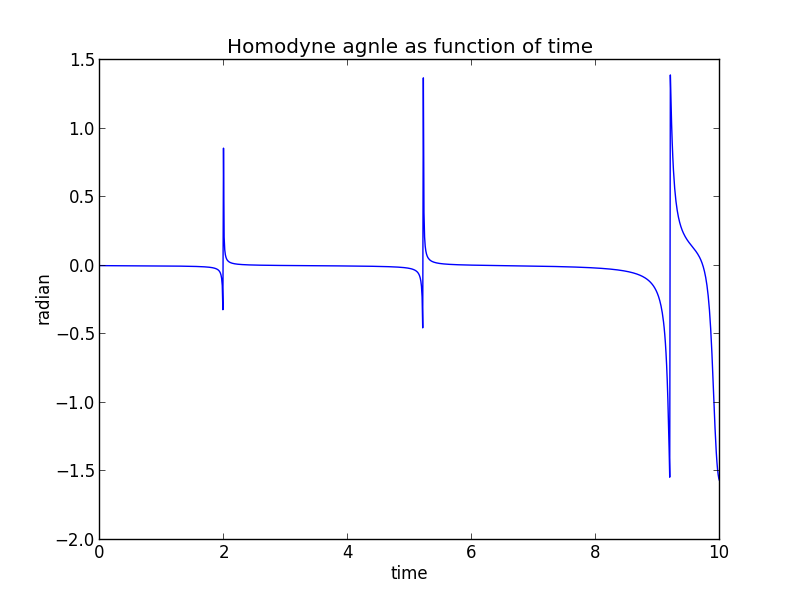
\includegraphics[width=1.\linewidth]{homodyne_angle_var}
 \end{minipage}
\hfill
 \begin{minipage}{0.45\linewidth}
  \center{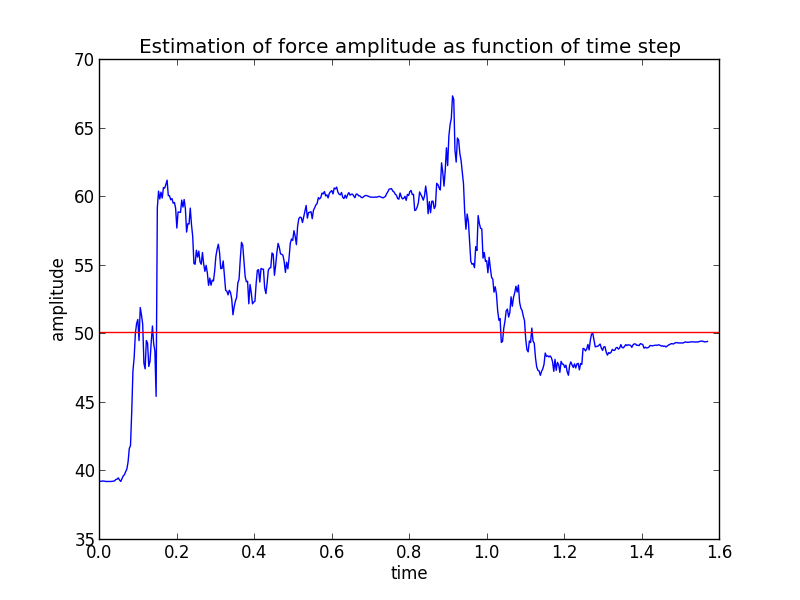
\includegraphics[width=1.\linewidth]{force_estimation}}
 \end{minipage}
\caption{Homodyne angle $\zeta(t)$ dependence of time \textit{(left)} and estimation of delay time depending on time \textit{(right)} (one period).}
\label{pic:hom}
\end{figure}
\begin{figure}
 \begin{minipage}{0.45\linewidth}
  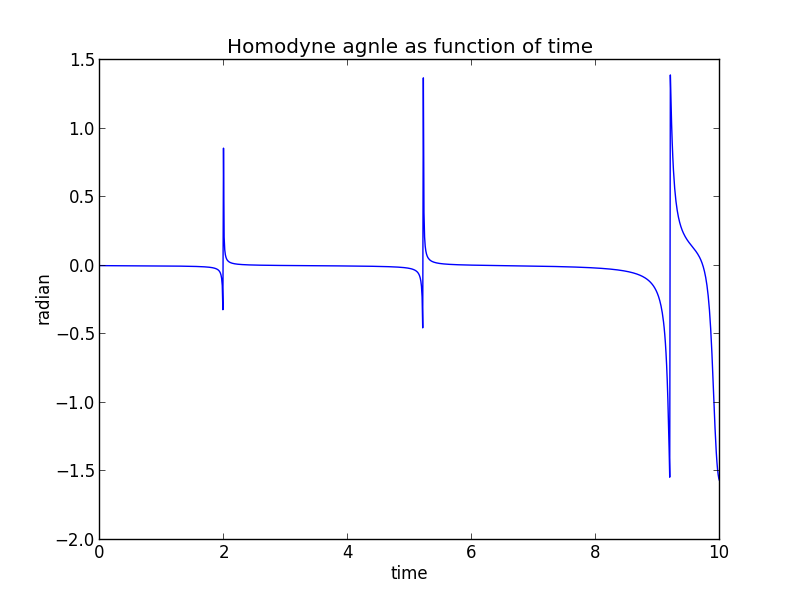
\includegraphics[width=1.\linewidth]{homodyne_angle_var}
 \end{minipage}
\hfill
 \begin{minipage}{0.45\linewidth}
  \center{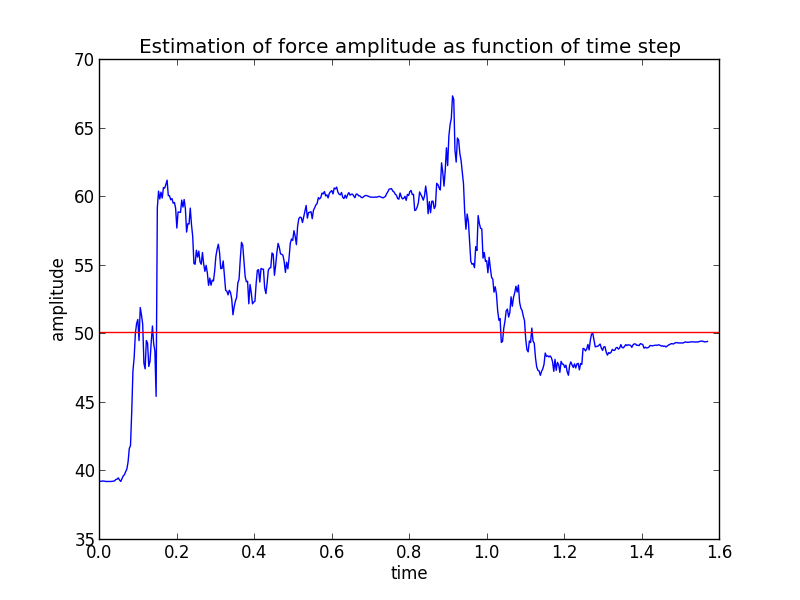
\includegraphics[width=1.\linewidth]{force_estimation}}
 \end{minipage}
\caption{Homodyne angle $\zeta(t)$ dependence of time \textit{(left)} and estimation of delay time depending on time \textit{(right)} (one period).}
\label{pic:filt}
\end{figure}
\end{document}